% vim: set sts=4 et :
\documentclass[aps,prd,reprint,nofootinbib,preprintnumbers]{revtex4}

\usepackage{amsfonts}
\usepackage{amsmath}
\usepackage{graphicx}
\usepackage[svgnames]{xcolor}
\usepackage{hepparticles}
\usepackage{hepnicenames}
\usepackage{hepunits}
\usepackage{graphicx}
\usepackage{caption}
\usepackage{subcaption}
\usepackage{epstopdf}
%% Shortcuts %%
\newcommand{\dd}{\text{d}}
\newcommand{\refapp}[1]{app.~(\ref{app:#1})}
\newcommand{\refeq}[1]{eq.~(\ref{eq:#1})}
\newcommand{\refsec}[1]{sec.~(\ref{sec:#1})}
\newcommand{\reftab}[1]{tab.~(\ref{tab:#1})}
\newcommand{\nuvec}{\vec{\nu}}
\newcommand{\thvec}{\vec{\vartheta}}
\let\oldtheta\theta
\renewcommand{\theta}{\vartheta}
%\newcommand{\GeV}{\text{GeV}}
\newcommand{\order}[1]{\mathcal{O}\left({#1}\right)}
\let\eps\varepsilon
\newcommand{\aver}[1]{\langle #1 \rangle}
\newcommand{\what}[1]{\widehat{#1}}
\newcommand{\wwhat}[1]{\widehat{\widehat{#1}}}
\DeclareMathOperator{\cov}{Cov}

%% Draft Macros %%
\newcommand{\todo}[1]{{\color{red}\bf ToDo: #1}}
\newcommand{\danny}[1]{{\color{purple}#1}}
\newcommand{\fred}[1]{{\color{brown!85!black}#1}}
\newcommand{\nico}[1]{{\color{green!85!black}#1}}
\newcommand{\citeneeded}{{\color{red}\bf [cite needed]}}

\begin{document}

\allowdisplaybreaks

\preprint{SI-HEP-2014-xx}
\title{Sample-Based Determination of Angular Observables}
\author{Frederik Beaujean}
\email{frederik.beaujean@lmu.de}
\affiliation{C2PAP, Universe Cluster, Ludwig-Maximilians-Universit\"at M\"unchen, Garching, Germany}
\author{Marcin Chrzaszcz}
\email{mchrzasz@cern.ch}
\author{Nicola Serra}
\email{nicola.serra@cern.ch}
\affiliation{Physik-Institut, Universit\"at Z\"urich, Z\"urich, Switzerland}
\author{Danny van Dyk}
\email{vandyk@tp1.physik.uni-siegen.de}
\affiliation{Theoretische Physik 1, Naturwissenschaftlich-Technische Fakult\"at,
Universit\"at Siegen, Siegen, Germany}

\begin{abstract}
In this letter we study how to obtain a set of angular observables
$\{P_i\}$ that arise in a generic multi-body process without the need
to carry out a likelihood fit of an angular distribution to the
measured events. Instead, we present a method that only relies on
orthogonality of angular functions, and estimation of integrals
by means of Monte Carlo techniques.
\end{abstract}

\maketitle

\section{Introduction}
\label{sec:intro}

The initial motivation for studying what we wish to call the \emph{Method of Moments}
is the determination of angular observables in the rare decay FCNC-mediated decay
$\bar{B}\to \bar{K}^*(\to \bar{K}\pi)\ell^+\ell^-$. However, we emphasize that
he method we describe in the remainder of this letter is general and applies to arbitrary
decay or scattering processes.\\

Let $\thvec = (\theta_1, \dots \theta_N)$ denote the set of all
angles, and let $\nuvec = (\nu_1, \dots \nu_M)$ denote the set of all
other non-angular kinematic variables needed to fully specify the
final state of the process under study. For example, $\nuvec$ may
include invariant masses or center-of-mass energies. We define an
angular observable $P_i$ as a coefficient in the probability density
function (PDF) of the process,
\begin{align}
    \label{eq:def-P}
    P(\nuvec, \thvec) = \sum_i P_i(\nuvec) \times f_i(\thvec)\,.
\end{align}
Here, the dependence on the $n$ decay angles $\thvec$ has been
explicitly factored out in terms of the angular functions
$f_i(\thvec)$, which we assume to fulfill the orthonormality relations
\begin{equation}
    \label{eq:def-ortho-rel}
    \int_\Omega f_i(\thvec) f_j(\thvec) \dd^N \theta = \delta_{ij}\,.
\end{equation}
For the purpose of this letter, however, it suffices that the system
of angular functions $f_i(\thvec)$ can be transformed into an
orthonormal basis. The transformation needs to be worked out on a
case-by-case basis. For a selection of $B$ decays, the transformations
are listed in the appendices \ref{app:btokll} through
\ref{app:lambdabtolambdall}.  Note that $P_i$ is \emph{not} a PDF.  \\


For particle decays, $P$ is generally expressed in terms of the fully differential decay width,
\begin{align}
    \label{eq:def-P-decay}
    P(\nuvec, \thvec) \equiv \frac{1}{\Gamma}\frac{\dd^{N+M}\Gamma}{\dd \nu_1 \dots \dd \nu_M\, \dd \theta_1 \dots \theta_N}\,,
\end{align}
where $\Gamma$ is the total decay width. For a scattering process, one can similarly use
\begin{align}
    \label{eq:def-P-scattering}
    P(\nuvec, \thvec) \equiv \frac{1}{\sigma}\frac{\dd^{N+M}\sigma}{\dd \nu_1 \dots \dd \nu_M\, \dd \theta_1 \dots \theta_N}\,,
\end{align}
where the total cross section $\sigma$ is used for the
normalization. Since the determination of the total decay width or
total cross section can be quite difficult, we emphasize that
different normalizations for $P$ can be used.  For instance, the total
decay width (or cross section) of the process of interest can be
replaced by the corresponding quantity of a control-channel
process.\fred{How would $P$ remain a proper probability such that
  $\int P = 1$? You can't simply change the normalization. I propose a
  change of notation: I find it terribly confusing that $P(\nuvec,
  \thvec)$ is a probability but $P_i(\nuvec)$ is not. For $P_i$, later
  on the symbols $J_i, K_i$ etc are used. We don't have to use the
  same symbol everywhere but let's not use $P_i$}\\


In the remainder of this letter we discuss how to obtain the angular
observables $P_i(\nuvec)$ in an experimental setup where each recorded
event is (approximately) distributed according to $P$.  We establish
the statistical basics in section \ref{sec:sample-based-det}. Section
\ref{sec:systematics} is dedicated to the impact of systematic effects
such as mismodeling the underlying physics or detector acceptance
effects. Numerical studies for one uni-angular and one triple-angular
distribution are provided in section \ref{sec:numerics}. In a series
of appendices we provide the orthonormal bases of angular functions
relevant to several rare $b$ decays.



\section{Sample-Based Determination}
\label{sec:sample-based-det}

The orthonormality relations \refeq{def-ortho-rel} imply that a single angular observable $P_i$
can be projected out of the full PDF $P$ by means of
\begin{equation}
    \label{eq:det-Pi-analytical}
    P_i(\nuvec) = \int_{\thvec = 0}^{2\pi} f_i(\thvec) P(\nuvec, \thvec) \dd^N \theta\,.
\end{equation}
In point of fact, $P_i$ is the $f_i$-th moment of the PDF $P$\fred{This
  notation is uncommon. Is that how we \emph{define} the $f_i$-th
  moment?}. Additionally, integration over the non-angular variables
yields
\begin{equation}
    \langle P_i\rangle
    \equiv \int P_i(\nuvec) \dd^M \nu
    = \int \left[\int_{\thvec=0}^{2\pi} f_i(\thvec) P(\nuvec,\thvec) \dd^N\theta\right]\dd^M \nu\,.
\end{equation}
The remainder of this section  describes the method of moments, in which we replace the
analytical integration \refeq{det-Pi-analytical} by Monte Carlo (MC) estimators.\\


The central tenet of MC integration is the fact that the expectation value $E_P[g]$ of some function
$g(x)$ under the probability density $P(x)$,
\begin{equation}
    E_P[g] \equiv \int g(x) P(x) \dd x
\end{equation}
can be approximated \cite{MCSM-2004} by an MC estimator $\what{E_P[g]}$
\begin{equation}
    \label{eq:mc-id}
    E_P[g] \to \widehat{E_P[g]} \equiv \frac{1}{K} \sum_{k=1} g(x^{(k)})
\end{equation}
due to the strong law of large numbers for $K \to \infty$ assuming
that the variates $x^{(k)}$, $k = 1, \dots, K$ are distributed as
$P$; i.e.,
\begin{equation}
    x^{(k)} \sim P\,.
\end{equation}
Throughout this letter we denote all MC estimators with a wide hat.\\


We assume, for a moment, that $P$ describes the distribution of the underlying
physical process truthfully. In that case, all events detected in an experimental setup are in fact, up to
detection efficiencies, distributed as $P$. \fred{Paragraph is redundant an can be omitted.}

Application of \refeq{mc-id} then yields \fred{notation is very confusing $P_i$ for $x^{(k)} \sim P$}
\begin{equation}
    \langle P_i\rangle \to \widehat{\langle P_i\rangle} = \frac{1}{K} \sum_{k=1}^{K} f_i(x^{(k)})\,.
\end{equation}
It is often of interest to obtain the $\nuvec$- observables integrated
over certain ranges of $\nuvec$; i.e., binned measurements of $\langle
P_i\rangle$
Therefore, we introduce the bin-integrated quantity
\begin{align}
    \langle P_i\rangle_{\vec{a},\vec{b}}
    & = \int_{\vec{a}}^{\vec{b}} P_i(\nuvec) \dd^M \nu\\
    & = \int_{\vec{a}}^{\vec{b}} \left[\int_{\thvec=0}^{2\pi} f_i(\thvec) P(\nuvec,\thvec) \dd^N\theta\right]\dd^M \nu\\
    & = \int \left[\int_{\thvec=0}^{2\pi} f_i(\thvec) P(\nuvec,\thvec)
        \mathbf{1}(\vec{a} \le \nuvec \le \vec{b})\,
        %% \theta^{(m)}(\nuvec - \vec{a}) \theta^{(m)}(\vec{b} - \nuvec)
        \dd^N\theta\right]\dd^M \nu\,,
\end{align}
where the argument of the indicator function $ \mathbf{1}(\vec{a} \le
\nuvec \le \vec{b})$ is to be interpreted componentwise.
Application of \refeq{mc-id} immediately yields
\begin{equation}
    \label{bin-importance}
    \widehat{\langle P_i\rangle_{\vec{a},\vec{b}}}
    = \frac{1}{K} \sum_{k=1}^{K} f_i(x^{(k)})         \mathbf{1}(\vec{a} \le \nuvec \le \vec{b})\,.
\end{equation}
This basically reduces the estimation of
$\aver{P_i}_{\vec{a},\vec{b}}$ to a (weighted) counting experiment. In
the limit $N \to \infty$, the random vector $( \dots,
\aver{P_i}_{\vec{a},\vec{b}}, \dots)$ follows a multivariate Gaussian
distribution \citeneeded\fred{Why?  multivariate in $\widehat{P_i}$?}
with a mean vector estimated by \refeq{bin-importance} and covariance
estimated as
\begin{equation}
    \cov[\aver{P_i},\aver{P_j}]_{\vec{a},\vec{b}} \to \what{\cov}[\aver{P}_i, \aver{P}_j]_{\vec{a},\vec{b}}
        = \frac{1}{K - 1} \sum_{k=1}^{K} \big[{f}_i(x^{(k)}) - \widehat{\langle P_i\rangle_{\vec{a},\vec{b}}}\big]\,\big[f_j(x^{(k)}) - \widehat{\langle P_j\rangle_{\vec{a},\vec{b}}}\big]
        \mathbf{1}(\vec{a} \le \nuvec \le \vec{b})\,.
\end{equation}
We would like to emphasize that the sample covariance should rapidly \fred{So what value of $K$ is close enought to $\infty$?} converge towards the true covariance matrix.
This will allow to construct constraints on optimized observables with correlated uncertainties
from the experimental constraints on the angular observables. (See \cite{Egede:2008uy,Egede:2010zc,Bobeth:2010wg,Becirevic:2011bp,Bobeth:2012vn,Matias:2012xw,DescotesGenon:2012zf}
for definitions of such optimized observables in $B\to K^*\ell^+\ell^-$ decays).



\section{Sources of Systematic Uncertainties}
\label{sec:systematics}

In \refsec{sample-based-det}, we assume that the PDF $P$ describe the physical reality accurately,
and that the experiment observes each event with perfect accuracy. In order to estimate systematic
uncertainties, we lift these assumptions.

\subsection{Mismodeling due to Contributions by Higher Partial Waves}
\label{sec:systematics:partial-waves}

\fred{Paragraph is very specific to one physics case. Needs a drawing}

So far, we assumed that our underlying physical process was accurately described by our PDF $P$.
However, in several interesting processes we might only have an approximative result for $P$.
We will now show that this is the case for the interesting class of four-body decays $B\to P_1 P_2 \ell_1 \bar\ell_2$,
which includes the rare $b\to s$-mediated $B$ decay $B \to K\pi\ell^+\ell^-$ and the $V_{ub}$ suppressed decay
$B\to \pi\pi\ell^+\bar\nu_\ell$. For both examples the PDF $P$ is known in the small-width approximation
and when assuming a pure $P$-wave, resonant final state. An extension to $S-P$ interference has been
studied for $B\to K\pi\ell^+\ell^-$ \cite{Blake:2012mb,Becirevic:2011bp} and for $\bar{B}\to \pi\pi\ell^-\bar\nu_\ell$
\cite{Faller:2013dwa}.

For this class of decays, we face the problem that $P$ has a given dependence on the dilepton helicity angle $\theta_1$
and the azimuthal angle $\theta_3$. (See also \refapp{btokpill} for details on the angular distribution.)
However, on the level of decay amplitudes the dimeson system can have an arbitrary
large total angular momentum; only the third component of its angular momentum is restricted to $J^{\pi\pi}_z = -1,0,+1$.\\

We advocate here that is a sensible procedure to perform an expansion in terms of Legendre polynomials $p_{j}^{(m)}$
with respect to the remaining angle $\theta_2$. Using the observables $P_k(\vec{\nu}=(q^2, k^2))$ as defined in \refapp{partial-waves}
the expansion reads
\begin{equation}
    P_{k}(\vec{\nu},\cos\theta_2) \equiv \sum_{j} \frac{1}{n_{j,m}} P_{k,j}(\vec{\nu}) p_{j}^{(m)}(\cos\theta_2)\sin\theta_2\,,
\end{equation}
where $m=0$ for $n=1,2,6$ and $m=1$ for $n=3,4,5,7,8,9$. The angular observables defined as coefficients of this expansion
have the merit of a well-defined total angular momentum, and thus can be disentangled for
a derivation). As a consequence of the orthogonality of the Legendre polynomials, mismodelling or lack of modelling of higher
partial-wave observables \emph{does not affect} the method of moments as given in the previous section.
Unfortunately, this benefit on the experimental side is accompanied with a theoretical draw back. Each observable
$P_{k,j}(\vec{\nu})$ consists of an infinite sum of bilinear of partial-wave amplitudes. It remains for theoretical
analyses to estimate or calculate the impact of partial waves beyond the S and P wave contributions. (For $B\to K\pi\ell^+\ell^-$ an initial study has been carried out for contributions up to the D wave \cite{Das:2014}).\\

We wish to emphasize, however, that detector acceptance effects systematically affect the expansion for any basis
of angular functions. The means to cope with this problem are discussed in the following subsection.


\subsection{Detector Acceptance Effects and Backgrounds}
\label{sec:systematics:acceptance}

\fred{If this is to be general, should explain what we mean by
  acceptance. Isn't it that experiments just model the detector well?
  The P. to observe an event in $\nuvec, \thvec$ might be very
  different from the P. to create an event in $\nuvec, \thvec$. All
  that's needed is a full forward model. I'm not sure that in
  \refeq{eq:PDFwithDE} we still have a normalized probability. Am I
  right to say that detector effects can be very much localized and
  nondifferentiable? Like some wires are inactive, or the region close
  to the beam has zero acceptance. In the latter case, modeling
  residual acceptance effects with smooth Legendre polynomials seems a
  bad idea.}

Thanks to accurate detector simulations and control studies, the experimental analyses have become
remarkably good at removing detector acceptance effects. In this section we therefore assume that
there are only a small, residual acceptance effects left that affect the events. In particular, we
assume that the latter can be modeled as a modified probability density,
\begin{equation}
    \label{eq:PDFwithDE}
    P(\nuvec,\thvec) \to P(\nuvec,\thvec) \times \Omega(\thvec),
\end{equation}
where $\Omega$ is independent of the non-angular kinematics $\nuvec$. The latter assumption is only
is invalid in general. However, if residual angular acceptance only weakly depends on $\vec{\nu}$, one
can always choose appropriate bin $\vec{\nu}$ so that $\Omega$ is approximately constant with respect
to $\vec{\nu}$. For such a case we parametrize
\begin{equation}
    \Omega_{m,l}(\thvec) = \prod_{i=1}^{m} \Big[1 + \sum_{j=1}^l \eps_i^{(j)} p_j(\cos\theta_i)\big]
\end{equation}
where $p_j(\cos\theta_i)$ denotes the $j$th Legendre polynomial. Since we only consider residual
acceptance effects, we expect $\eps_i^{(j)} \ll 1$. \footnote{\danny{what are reasonable values/upper limits on the $\eps$?}}\\

We are aware that setting a bin width that fulfills the aforementioned criterion can be at odds with
other requirements. For instance, in exclusive $b\to s\ell^+\ell^-$ decays, the bin width for
$\vec{\nu} = q^2$ needs to cover a sufficiently large part of the phase space beyond the open charm
threshold. We emphasize that the outcome of an analysis as proposed here can easily combine several
bins by means of a weighted average.\\

\paragraph{Uniangular Distribution}
For definiteness and clarity, we consider first an uni-angular distribution $P(\theta)$.
In this case we can parametrize the PDF $P$ as
\begin{equation}
    P(\theta) = P_1 + P_2 \cos\theta + P_2 \cos^2\theta\,,
\end{equation}
which is a parametrization that has been used in the literature for $\bar{B}\to\bar{K}\ell^+\ell^-$ decays \cite{Bobeth:2007dw}.
While this system of angular functions is not orthonormal, it can easily be orthonormalized. For the basis of angular
functions, see \refapp{btokll}.
Considering detector acceptance effects up to second order in $\cos\theta$, the function $\Omega(\vec\theta)$ reads
\begin{equation}
    \Omega_{1,2}(\theta_1) = 1 + \eps_{1}^{(1)} \cos\theta + \frac{\eps_{1}^{(2)}}{2}\big(3 \cos^2\theta - 1\big)\qquad\eps_{1}^{(i)} = \order{\eps}\,.
\end{equation}
Inclusion of $\Omega_{1,2}$ as part of the PDF as proposed in \refeq{PDFwithDE} modifies the MC estimators for the angular observables.
We find
\begin{equation}
\begin{aligned}
    \wwhat{P_1} & = \Big(1 + \frac{\eps_{1}^{(2)}}{2}\Big) \what{P_1} + \frac{9 \eps_{1}^{(2)}}{70} \what{P_3}\\
    \wwhat{P_2} & = \Big(1 - \frac{2 \eps_{1}^{(2)}}{5}\Big) \what{P_2} - \eps_{1}^{(1)} \what{P_1} - \frac{3\eps_{1}^{(1)}}{5} \what{P_3}\\
    \wwhat{P_3} & = \Big(1 - \frac{11\eps_{1}^{(2)}}{14}\Big)\what{P_3} - \frac{3\eps_{1}^{(2)}}{2} \what{P_1} - \eps_{1}^{(1)} \what{P_2}\,.
\end{aligned}
\end{equation}
Here $\what{P_i}$ denotes the uncorrected estimators, while $\wwhat{P_i}$ denotes the efficiency-corrected estimators of the angular observables.\\

\paragraph{Triangular Distribution}

\begin{table*}
    \resizebox{.99\textwidth}{!}{\ensuremath{\left(
\begin{array}{cccccc}
 \frac{13}{35} \eps_{1}^{(2)}-\frac{1}{4} \eps_{2}^{(2)}-\frac{1}{4} \eps_{3}^{(2)} & \frac{9}{70} \eps_{1}^{(2)} & 0 & -\frac{39}{140} \eps_{2}^{(2)} & 0 & 0 \\
 -\frac{12}{35} \eps_{1}^{(2)} & -\frac{23}{35} \eps_{1}^{(2)}-\frac{1}{4} \eps_{2}^{(2)}-\frac{1}{4} \eps_{3}^{(2)} & -\eps_{1}^{(1)} & 0 & -\frac{39}{140} \eps_{2}^{(2)} & 0 \\
 -\frac{2}{5} \eps_{1}^{(1)} & -\frac{3}{5} \eps_{1}^{(1)} & -\frac{2}{5} \eps_{1}^{(2)}-\frac{1}{4} \eps_{2}^{(2)}-\frac{1}{4} \eps_{3}^{(2)} & 0 & 0 & -\frac{39}{140} \eps_{2}^{(2)} \\
 -\frac{3}{4} \eps_{2}^{(2)} & 0 & 0 & \frac{13}{35} \eps_{1}^{(2)}-\frac{1}{28} \eps_{2}^{(2)}-\frac{1}{4} \eps_{3}^{(2)} & \frac{9}{70} \eps_{1}^{(2)} & 0 \\
 0 & -\frac{3}{4} \eps_{2}^{(2)} & 0 & -\frac{12}{35} \eps_{1}^{(2)} & -\frac{23}{35} \eps_{1}^{(2)}-\frac{1}{28} \eps_{2}^{(2)}-\frac{1}{4} \eps_{3}^{(2)} & -\eps_{1}^{(1)} \\
 0 & 0 & -\frac{3}{4} \eps_{2}^{(2)} & -\frac{2}{5} \eps_{1}^{(1)} & -\frac{3}{5} \eps_{1}^{(1)} & -\frac{2}{5} \eps_{1}^{(2)}-\frac{1}{28} \eps_{2}^{(2)}-\frac{1}{4} \eps_{3}^{(2)} \\
 -\frac{15}{16} \eps_{3}^{(2)} & -\frac{15}{64} \eps_{3}^{(2)} & 0 & \frac{9}{16} \eps_{3}^{(2)} & \frac{9}{64} \eps_{3}^{(2)} & 0 \\
 0 & 0 & 0 & 0 & 0 & 0 \\
 0 & 0 & 0 & 0 & 0 & 0 \\
 0 & 0 & -\frac{45}{512} \pi ^2 \eps_{3}^{(1)} & 0 & 0 & \frac{45 \pi ^2 \eps_{3}^{(1)}}{1024} \\
 -\frac{27}{256} \pi ^2 \eps_{3}^{(1)} & -\frac{9}{256} \pi ^2 \eps_{3}^{(1)} & 0 & \frac{27}{512} \pi ^2 \eps_{3}^{(1)} & \frac{9}{512} \pi ^2 \eps_{3}^{(1)} & 0 \\
 -\eps_{2}^{(1)} & 0 & 0 & -\frac{1}{5} \eps_{2}^{(1)} & 0 & 0 \\
 0 & -\eps_{2}^{(1)} & 0 & 0 & -\frac{1}{5} \eps_{2}^{(1)} & 0 \\
 0 & 0 & 0 & 0 & 0 & 0 \\
 0 & 0 & 0 & 0 & 0 & 0 \\
 0 & 0 & 0 & 0 & 0 & 0 \\
 0 & 0 & 0 & 0 & 0 & 0 \\
 0 & 0 & 0 & 0 & 0 & 0 \\
\end{array}
\right)
}}\\[2.5\medskipamount]
    \resizebox{.99\textwidth}{!}{\ensuremath{\left(
\begin{array}{cccccc}
 -\frac{3}{16} \eps_{3}^{(2)} & 0 & 0 & 0 & -\frac{567 \pi ^2 \eps_{3}^{(1)}}{16384} & -\frac{1}{2} \eps_{2}^{(1)} \\
 0 & 0 & 0 & 0 & -\frac{81 \pi ^2 \eps_{3}^{(1)}}{8192} & 0 \\
 0 & 0 & 0 & -\frac{81 \pi ^2 \eps_{3}^{(1)}}{2048} & 0 & 0 \\
 \frac{3}{16} \eps_{3}^{(2)} & 0 & 0 & 0 & \frac{315 \pi ^2 \eps_{3}^{(1)}}{16384} & -\frac{1}{2} \eps_{2}^{(1)} \\
 0 & 0 & 0 & 0 & \frac{45 \pi ^2 \eps_{3}^{(1)}}{8192} & 0 \\
 0 & 0 & 0 & \frac{45 \pi ^2 \eps_{3}^{(1)}}{2048} & 0 & 0 \\
 \frac{2}{7} \eps_{1}^{(2)}+\frac{2}{7} \eps_{2}^{(2)}-\frac{1}{4} \eps_{3}^{(2)} & 0 & 0 & 0 & -\frac{2025 \pi ^2 \eps_{3}^{(1)}}{32768} & 0 \\
 0 & -\frac{1}{7} \eps_{1}^{(2)}-\frac{1}{7} \eps_{2}^{(2)}-\frac{5}{8} \eps_{3}^{(2)} & -\frac{1}{2} \eps_{1}^{(1)} & -\frac{1}{2} \eps_{2}^{(1)} & 0 & 0 \\
 0 & -\frac{2}{5} \eps_{1}^{(1)} & \frac{1}{5} \eps_{1}^{(2)}-\frac{1}{7} \eps_{2}^{(2)}-\frac{5}{8} \eps_{3}^{(2)} & 0 & -\frac{1}{2} \eps_{2}^{(1)} & -\frac{135 \pi ^2 \eps_{3}^{(1)}}{2048} \\
 0 & -\frac{2}{5} \eps_{2}^{(1)} & 0 & -\frac{1}{7} \eps_{1}^{(2)}+\frac{1}{5} \eps_{2}^{(2)}-\frac{5}{8} \eps_{3}^{(2)} & -\frac{1}{2} \eps_{1}^{(1)} & 0 \\
 -\frac{81 \pi ^2 \eps_{3}^{(1)}}{2048} & 0 & -\frac{2}{5} \eps_{2}^{(1)} & -\frac{2}{5} \eps_{1}^{(1)} & \frac{1}{5} \eps_{1}^{(2)}+\frac{1}{5} \eps_{2}^{(2)}-\frac{5}{8} \eps_{3}^{(2)} & 0 \\
 0 & 0 & -\frac{63 \pi ^2 \eps_{3}^{(1)}}{1024} & 0 & 0 & \frac{13}{35} \eps_{1}^{(2)}-\frac{2}{5} \eps_{2}^{(2)}-\frac{1}{4} \eps_{3}^{(2)} \\
 0 & 0 & -\frac{9}{512} \pi ^2 \eps_{3}^{(1)} & 0 & 0 & -\frac{12}{35} \eps_{1}^{(2)} \\
 0 & 0 & 0 & 0 & 0 & 0 \\
 0 & 0 & 0 & 0 & 0 & 0 \\
 0 & 0 & 0 & 0 & 0 & 0 \\
 0 & 0 & 0 & 0 & 0 & 0 \\
 0 & 0 & 0 & 0 & 0 & 0 \\
\end{array}
\right)
}}\\[2.5\medskipamount]
    \resizebox{.99\textwidth}{!}{\ensuremath{\left(
\begin{array}{cccccc}
 0 & 0 & 0 & 0 & 0 & 0 \\
 -\frac{1}{2} \eps_{2}^{(1)} & 0 & 0 & 0 & 0 & 0 \\
 0 & 0 & 0 & 0 & 0 & 0 \\
 0 & 0 & 0 & 0 & 0 & 0 \\
 -\frac{1}{2} \eps_{2}^{(1)} & 0 & 0 & 0 & 0 & 0 \\
 0 & 0 & 0 & 0 & 0 & 0 \\
 0 & 0 & 0 & 0 & 0 & 0 \\
 0 & 0 & 0 & 0 & 0 & 0 \\
 -\frac{45 \pi ^2 \eps_{3}^{(1)}}{2048} & 0 & 0 & 0 & 0 & 0 \\
 0 & 0 & 0 & 0 & 0 & 0 \\
 0 & 0 & 0 & 0 & 0 & 0 \\
 \frac{9}{70} \eps_{1}^{(2)} & 0 & 0 & 0 & 0 & 0 \\
 -\frac{23}{35} \eps_{1}^{(2)}-\frac{2}{5} \eps_{2}^{(2)}-\frac{1}{4} \eps_{3}^{(2)} & 0 & 0 & 0 & 0 & 0 \\
 0 & -\frac{1}{7} \eps_{1}^{(2)}+\frac{1}{5} \eps_{2}^{(2)}+\frac{1}{8} \eps_{3}^{(2)} & -\frac{1}{2} \eps_{1}^{(1)} & -\frac{2}{5} \eps_{2}^{(1)} & 0 & 0 \\
 0 & -\frac{2}{5} \eps_{1}^{(1)} & \frac{1}{5} \eps_{1}^{(2)}+\frac{1}{5} \eps_{2}^{(2)}+\frac{1}{8} \eps_{3}^{(2)} & 0 & -\frac{2}{5} \eps_{2}^{(1)} & -\frac{81 \pi ^2 \eps_{3}^{(1)}}{2048} \\
 0 & -\frac{1}{2} \eps_{2}^{(1)} & 0 & -\frac{1}{7} \eps_{1}^{(2)}-\frac{1}{7} \eps_{2}^{(2)}+\frac{1}{8} \eps_{3}^{(2)} & -\frac{1}{2} \eps_{1}^{(1)} & 0 \\
 0 & 0 & -\frac{1}{2} \eps_{2}^{(1)} & -\frac{2}{5} \eps_{1}^{(1)} & \frac{1}{5} \eps_{1}^{(2)}-\frac{1}{7} \eps_{2}^{(2)}+\frac{1}{8} \eps_{3}^{(2)} & 0 \\
 0 & 0 & -\frac{2025 \pi ^2 \eps_{3}^{(1)}}{32768} & 0 & 0 & \frac{2}{7} \eps_{1}^{(2)}+\frac{2}{7} \eps_{2}^{(2)}-\frac{1}{4} \eps_{3}^{(2)} \\
\end{array}
\right)
}}
    \caption{The matrix $N_{ij}$ that appears in \refeq{eff-corrected-est-btokstarll}. Due to spatial
        constraints, we split its display into columns $j=1s,1c,1i,2s,2c,2i$ (top),
        $j=3,4,4i,5,5i,6s$ (middle) and $j=6c,7,7i,8,8i,9$ (bottom).
        \label{tab:eff-corrected-est-btokstarll}
    }
\end{table*}

As an example for a triangular distribution we use the decay $\bar{B}\to\bar{K}^*(\to \bar{K}\pi)\ell^+\ell^-$.
A parametrization of its angular distribution can be found in \refapp{btokstarll}.\\

For this type of distribution, we expand $\Omega_3$ to linear order in $\eps$,
\begin{equation}
    \Omega_{3,2}(\theta_1,\theta_2,\theta_3) = 1 + \sum_{i=1}^3 \sum_{j=1}^2 \eps_i^{(j)} p_j(\cos\theta_i) + \order{\eps^2}\,.
\end{equation}
This leads to a matrix-valued equation that relates the effiency-corrected estimators $\wwhat{P}_i$ to the uncorrected
estimators $\what{P}_j$,
\begin{equation}
    \label{eq:eff-corrected-est-btokstarll}
    \wwhat{P}_i = \sum_{j=1\text{s},\dots\,9} \big(\delta_{ij} + N_{ij}\big) \what{P}_j\,.
\end{equation}
We provide the matrix $N$ in \reftab{eff-corrected-est-btokstarll}.\\

\paragraph{Recipe to determine the acceptance effects}

The determination of the coefficients $\eps_i^{(j)}$ that parametrize the detectory effects is generally
a difficult task. Here, we will show a systematic method to determine these coefficients.\\
One starts from generating a flap phase space MonteCarlo sample. Simulated events are then put thought the detector simulation, and selection requirements. Since flap phase space ensures flat distribution of angles on the generated level, the only non zero moment is one associated to Fl. Measuring the moments of this MC sample leads will etc. Mayby this should be an appendix.





\section{Toy Studies}
\label{sec:numerics}







\todo{
\begin{itemize}
    \item Simulate this for one angle $\theta_{1}$ (similar to $B\to K \ell^+\ell^-$) with varying samples sizes.
    \item Simulate this for three angles $\theta_{1\dots 3}$ (similar to $B\to K^*(\to K \pi)\ell^+\ell^-$) with varying samples sizes.
    \item Also, check explicitly the variance and covariance of the results for all sample sizes considered.
    \item compare robustness to likelihood fit when fit doesn't
      converge. Why exactly doesn't it converge? What if physics model
      wrong, say some angular terms are missing.
\end{itemize}}


\section{Conclusion}

In this letter \dots
\begin{enumerate}
    \item errors on the means are in very good approximation gaussian.
    \item correlation are small and faithfully model a multivariate gaussian. \fred{$\Rightarrow$ easy transfer of knowledge to theory fits}
\end{enumerate}


\acknowledgments

The work of D.v.D has been supported by the Bundesministerium f\"ur Bildung und Forschung (BMBF).
\dots
\danny{Potential people to read the manuscript: Jochen Dingfelder (Belle-II, Bonn), Ulrik Egede (LHCb, Imperial London), Christoph Langenbruch (LHCb, Warwick), Michel De Cian (LHCb, Heidelberg), Adrian Bevan (ATLAS, Queen Mary)  }
D.v.D would like to thank Gudrun Hiller and Martin Jung for discussing the results of \cite{Das:2014xx} prior to publication.

\appendix

\section{Application to $\bar{B}\to\bar{K}\ell^+\ell^-$}
\label{app:btokll}

The PDF for the decay $\bar{B}\to\bar{K}\ell^+\ell^-$ has been calculated for the most
complete basis of dimension-six $b\to s \ell^+\ell^-$ operators. It reads \cite{Bobeth:2007dw,Bobeth:2012vn}
\begin{equation}
    P(q^2, \cos\theta_1) = \frac{1}{\Gamma} \frac{\dd^4\Gamma}{\dd q^2\,\dd \cos\theta_1} = \frac{a(q^2)}{\Gamma} + \frac{b(q^2)}{\Gamma} \cos\theta_1 + \frac{c(q^2)}{\Gamma} \cos^2\theta_1 = \sum_i P_i f_i(\cos\theta_1)\,,
\end{equation}
where the basis of angular functions $f_i$ reads
\begin{equation}
\begin{aligned}
    f_1 & = 1\,, &
    f_2 & = \cos\theta_1\,, &
    f_2 & = \cos^2\theta_1\,.
\end{aligned}
\end{equation}
Here we denote the dilepton mass squared as $q^2$, and the dilepton helicity angle as $\theta_1 \equiv \theta_{\ell}$. We transform the PDF from a $\cos\theta_1$-dependence
to a $\theta_1$-dependence \fred{why? Formula easier? Where is the ``-'' sign from the Jacobian $\partial_{\theta} \cos \theta = - \sin \theta$ },
\begin{equation}
    P(q^2, \theta_1) = \sum_i P_i f_i(\cos\theta_1) \sin \theta_1\,.
\end{equation}

We provide dual basis $\hat{f}_i$ of angular functions which is dual to the basis $f_i$ in the sense that \fred{What are the upper limits? $\pi$ or $2 \pi$? Not consistent with section I and II. I think it would be fair to talk about the dual basis already there. Do we set $f=0$ on $[\pi, 2 \pi]$?}
\begin{equation}
    \int_0^\pi \dd\theta_1 \hat{f}_i(\theta_1) f_j(\theta_1) \sin\theta_1 = \delta_{ij}\,,
\end{equation}
thereby enabling us to project out exactly one of the angular
observables $P_i(q^2)$
\begin{equation}
    \int_0^\pi \dd \theta_1\hat{f}_i(\theta_1) P(q^2, \theta_1) = P_i(q^2)\,.
\end{equation}
The dual basis reads
\begin{equation}
\begin{aligned}
    \hat{f}_1 & = \frac{9}{8} - \frac{15}{8}\cos^2\theta_1\,, &
    \hat{f}_2 & = \frac{3}{2}\cos\theta_1\,, &
    \hat{f}_3 & = -\frac{15}{8} + \frac{45}{8}\cos^2\theta_1\,.
\end{aligned}
\end{equation}

\section{Application to $\bar{B}\to\bar{K}\pi\ell^+\ell^-$ (S-wave and P-wave)}
\label{app:btokstarll}

The PDF for the decay $\bar{B}\to\bar{K}\pi\ell^+\ell^-$ -- up to and including P-wave contributions -- has been calculated
for the most general basis of dimension-six $b\to s$ operators. It reads \cite{Blake:2012mb,Bobeth:2012vn}\fred{In the theory convention. Now we use $J_i$ instead of $P_i$.}
\begin{equation}
    P(q^2, \cos\theta_1, \cos\theta_2, \phi) = \frac{1}{\Gamma} \frac{\dd^4\Gamma}{\dd q^2\,\dd \cos\theta_1\,\dd \cos\theta_2\,\dd \phi} = \frac{3}{8\pi} \sum_i \frac{J_{i}(q^2)}{\Gamma} f_i(\cos\theta_1, \cos\theta_2, \phi)\,,
\end{equation}
where $\theta_1 \equiv \theta_\ell$ is the dilepton helicity angle, and $\theta_2 \equiv \theta_{K^*}$ is the $\bar{K}\pi$ helicity angle.\fred{$\phi$ not explained}
The decay width is
\begin{equation}
    \Gamma = \frac{\big(3 J_{1c} - J_{2c}\big) + 2\big(3J_{1s} - J_{2s}\big)}{3}\,.
\end{equation}
The angular functions read \cite{Blake:2012mb,Bobeth:2012vn}
\begin{equation}
\begin{aligned}
    f_{1s} & = \sin^2\theta_2 &
    f_{1c} & = \cos^2\theta_2 &
    f_{1i} & = \cos\theta_2\\
    f_{2s} & = \sin^2\theta_2 \cos 2\theta_1 &
    f_{2c} & = \cos^2\theta_2 \cos 2\theta_1 &
    f_{2i} & = \cos\theta_2 \cos 2\theta_1\\
    f_{3}  & = \sin^2\theta_2\sin^2\theta_1 \cos 2\phi &
    f_{9}  & = \sin^2\theta_2\sin^2\theta_1 \sin 2\phi\\
    f_{4}  & = \sin 2\theta_2 \sin 2\theta_1 \cos\phi & & &
    f_{4i} & = \sin\theta_2 \sin 2\theta_1 \cos\phi\\
    f_{5}  & = \sin 2\theta_2 \sin \theta_1 \cos\phi & & &
    f_{5i} & = \sin\theta_2 \sin \theta_1 \cos\phi\\
    f_{6s} & = \sin^2\theta_2 \cos\theta_1 &
    f_{6c} & = \cos^2\theta_2 \cos\theta_1\\
    f_{7}  & = \sin 2\theta_2 \sin \theta_1 \sin\phi & & &
    f_{7i} & = \sin\theta_2 \sin \theta_1 \sin\phi\\
    f_{8}  & = \sin 2\theta_2 \sin 2\theta_1 \sin\phi & & &
    f_{8i} & = \sin\theta_2 \sin 2\theta_1 \sin\phi\,.
\end{aligned}
\end{equation}
We indicate contributions from the interference of S waves and P waves by an index \emph{i}. In terms of the angles $\theta_1$ and $\theta_2$, instead of their cosines, the PDF reads
\begin{equation}
    P(q^2, \theta_1, \theta_2, \phi) = \frac{3}{8\pi} \sum_i P_i(q^2) f_i(\cos\theta_1, \cos\theta_2, \phi) \sin\theta_1 \sin\theta_2\,,
\end{equation}
where we also define $P_i(q^2) = J_i(q^2) / \Gamma$.\\

We provide dual basis $\hat{f}_i$ of angular functions which is dual to the basis $f_j$ in the sense that
\begin{equation}
    \frac{3}{8\pi}\int_0^\pi \dd\theta_1 \int_0^\pi\,\dd\theta_2\, \int_0^{2\pi}\dd \phi \hat{f}_i(\theta_1,\theta_2,\phi) f_j(\theta_1,\theta_2,\phi) \sin\theta_1 \sin\theta_2 = \delta_{ij}\,,
\end{equation}
thereby enabling us to project out exactly one of the angular
observables $P_i(q^2)$
\begin{equation}
    \int_0^\pi \dd\theta_1 \int_0^\pi\,\dd\theta_2\, \int_0^{2\pi}\dd \phi \hat{f}_i(\theta_1,\theta_2,\phi) P(q^2, \theta_1,\theta_2,\phi) = P_i(q^2)\,.
\end{equation}
The dual basis reads
\begin{equation}
\begin{aligned}
    \hat{f}_{1s} & = \frac{\big( 63 \sin^2\theta_1 - 42 \cos^2\theta_1\big) + \big(  45 \sin^2\theta_1 - 30 \cos^2\theta_1\big)\cos 2\theta_2}{64} \,,\\
    \hat{f}_{1c} & = \frac{\big(-21 \sin^2\theta_1 + 84 \cos^2\theta_1\big) + \big( -15 \sin^2\theta_1 + 60 \cos^2\theta_1\big)\cos 2\theta_2}{32} \,,\\
    \hat{f}_{2s} & = \frac{\big( 45 \sin^2\theta_1 - 30 \cos^2\theta_1\big) + \big(+135 \sin^2\theta_1 - 90 \cos^2\theta_1\big)\cos 2\theta_2}{64} \,,\\
    \hat{f}_{2c} & = \frac{\big(-15 \sin^2\theta_1 + 60 \cos^2\theta_1\big) + \big( -45 \sin^2\theta_1 +180 \cos^2\theta_1\big)\cos 2\theta_2}{32} \,,
\end{aligned}
\end{equation}
as well as
\begin{equation}
\begin{aligned}
    \hat{f}_{1sc}& = \frac{\big(21 + 15 \cos2\theta_2\big)\cos\theta_1}{16}               \,,&
    \hat{f}_{2sc}& = \frac{\big(15 + 45 \cos2\theta_2\big)\cos\theta_1}{16}               \,,\\
    \hat{f}_{6s} & = \frac{\big( 9\sin^2\theta_1 -  6 \cos^2\theta_1\big)\cos\theta_2}{4} \,,&
    \hat{f}_{6c} & = \frac{\big(-3\sin^2\theta_1 + 12 \cos^2\theta_1\big)\cos\theta_2}{2} \,,\\
    \hat{f}_{3}  & = \frac{75 \sin^2\theta_1 \sin^2\theta_2 \cos2\phi}{32}                \,,&
    \hat{f}_{9}  & = \frac{75 \sin^2\theta_1 \sin^2\theta_2 \sin2\phi}{32}                \,,\\
    \hat{f}_{4}  & = \frac{75 \sin 2\theta_1 \sin 2\theta_2 \cos \phi}{32}                \,,&
    \hat{f}_{4i} & = \frac{15 \sin  \theta_1 \sin 2\theta_2 \cos \phi}{8}                 \,,\\
    \hat{f}_{5}  & = \frac{15 \sin 2\theta_1 \sin  \theta_2 \cos \phi}{8}                 \,,&
    \hat{f}_{5i} & = \frac{3  \sin  \theta_1 \sin  \theta_2 \cos \phi}{2}                 \,,\\
    \hat{f}_{7}  & = \frac{15 \sin 2\theta_1 \sin  \theta_2 \sin \phi}{8}                 \,,&
    \hat{f}_{7i} & = \frac{3  \sin  \theta_1 \sin  \theta_2 \sin \phi}{2}                 \,,\\
    \hat{f}_{8}  & = \frac{75 \sin 2\theta_1 \sin 2\theta_2 \sin \phi}{32}                \,,&
    \hat{f}_{8i} & = \frac{15 \sin  \theta_1 \sin 2\theta_2 \sin \phi}{8}                 \,.
\end{aligned}
\end{equation}

\section{Application to $\bar{B}\to P_1 P_2\ell^+\ell^-$ (all partial waves)}
\label{app:btokpill}

The class of $P\to P_1 P_2 \ell_1\bar\ell_2$ decays, where $P,P_1$, and $P_2$ are pseudoscalar mesons,
and $\ell_1$ and $\bar\ell_2$ are charged or neutral leptons, includes decays
such as $\bar{B}\to\bar{K}\pi\ell^+\ell^-$ and $\bar{B}\to \pi\pi\ell^-\bar\nu_\ell$. \fred{If this appendix includes the previous one, how come there are less angular functions here?}
Their PDFs can generally be written as \cite{Lee:1992ih}
\begin{equation}
    P(q^2, k^2, \cos\theta_1, \cos \theta_2, \phi) = \frac{1}{\langle \Gamma\rangle}\frac{\dd^5 \Gamma}{\dd q^2\,\dd k^2\, \dd\cos\theta_1\,\dd\cos\theta_2\,\dd\phi} = \frac{1}{4\pi} \sum_i \frac{I_i(q^2, k^2, \cos\theta_2)}{\Gamma} f_i(\cos\theta_1,\phi)\,,
\end{equation}
where
\begin{equation}
\begin{aligned}
    f_1 & = 1\,,              &
    f_2 & = \cos 2\theta_1\,, &
    f_6 & = \cos  \theta_1\,, \\
    f_3 & = \sin^2\theta_1 \cos 2\phi\,,&
    f_4 & = \sin 2\theta_1 \cos  \phi\,,&
    f_5 & = \sin  \theta_1 \cos  \phi\,,\\
    f_9 & = \sin^2\theta_1 \sin 2\phi\,.&
    f_8 & = \sin 2\theta_1 \sin  \phi\,,&
    f_7 & = \sin  \theta_1 \sin  \phi\,,
\end{aligned}
\end{equation}
Here we denote dilepton mass squared and the dilepton helicity angle as $q^2$ and $\theta_1$, while
the dimeson mass squared and the dimeson helicity angles are denoted as $k^2$ and $\theta_2$. The
azimuthal angle is denoted as $\phi$. The total decay width is
\begin{equation}
    \langle \Gamma\rangle = \int_0^\pi \dd\theta_1\,\dd q^2\,\dd k^2\,\sin\theta_2 \frac{3I_1(q^2, k^2, \cos\theta_2) - I_2(q^2, k^2, \cos\theta_2)}{3}\,.
\end{equation}
As usual, we transform from a $\cos\theta_1$-dependence to a $\theta_1$-dependence.
\begin{equation}
\begin{aligned}
    P(q^2, k^2, \theta_1, \theta_2, \phi)
    & = \frac{1}{4\pi} \sum_i \frac{I(q^2, k^2, \cos\theta_2)}{\Gamma} f_i(\theta_1, \phi) \sin\theta_1 \sin\theta_2\\
    & \equiv \frac{1}{4\pi} \sum_i P_i(q^2, k^2, \theta_2) f_i(\theta_1, \phi)\,.
\end{aligned}
\end{equation}
where we also define $P_i(q^2, k^2, \theta_2) \equiv \sin\theta_2 I_i(q^2, k^2, \cos\theta_2) / \Gamma$.\\

We provide a basis $\hat{f}_i$ of angular functions which is dual to the basis $f_j$ in the sense that
\begin{equation}
    \frac{1}{4\pi}\int_0^\pi \dd\theta_1 \int_0^{2\pi}\dd \phi \hat{f}_i(\theta_1,\phi) f_j(\theta_1,\phi) \sin\theta_1 = \delta_{ij}\,,
\end{equation}
thereby enabling us to project out exactly one of the angular
observables $P_i(q^2, k^2, \theta_2)$
\begin{equation}
    \int_0^\pi \dd\theta_1 \int_0^{2\pi}\dd \phi \hat{f}_i(\theta_1,\phi) P(q^2, k^2, \theta_1,\theta_2,\phi) = P_i(q^2, k^2, \theta_2)\,.
\end{equation}
The dual basis reads
\begin{equation}
\begin{aligned}
    \hat{f}_1 & = \frac{21 + 15 \cos 2\theta_1}{16}\,, &
    \hat{f}_2 & = \frac{15 + 45 \cos 2\theta_1}{16}\,, &
    \hat{f}_6 & = 3 \cos\theta_1                   \,, \\
    \hat{f}_3 & = \frac{15}{4}                \cos 2\phi     \,, &
    \hat{f}_4 & = \frac{15}{4} \sin 2\theta_1 \cos  \phi     \,, &
    \hat{f}_5 & = 3            \sin  \theta_1 \cos  \phi     \,, \\
    \hat{f}_9 & = \frac{15}{4}                \sin 2\phi     \,, &
    \hat{f}_8 & = \frac{15}{4} \sin 2\theta_1 \sin  \phi     \,, &
    \hat{f}_7 & = 3            \sin  \theta_1 \sin  \phi     \,.
\end{aligned}
\end{equation}


\section{Application to $\Lambda_b\to \Lambda(\to N \pi)\ell^+\ell^-$}
\label{app:lambdabtolambdall}

The physical PDF for the decay -- in the presence of Standard Model operator and their chirality flipped counter parts -- reads \cite{Boeer:2014xx}
\begin{equation}
    P_{\Lambda_b}(q^2, \cos\theta_1, \cos\theta_2, \phi) = \frac{1}{\Gamma} \frac{\dd^4\Gamma}{\dd q^2\,\dd \cos\theta_1\,\dd \cos\theta_2\,\dd \phi} = \frac{3}{8\pi} \sum_i \frac{K_{i}(q^2)}{\Gamma} f_i(\cos\theta_1, \cos\theta_2, \phi)\,,
\end{equation}
where $q^2$ denotes the dilepton mass squared, and $\theta_1 \equiv \theta_\ell$ and $\theta_2 \equiv \theta_\Lambda$ denote the
helicity angles in the dilepton and $N\pi$ systems, respectively. The basis of angular functions reads \fred{cite Danny's upcoming paper}
\begin{equation}
    \begin{aligned}
% 1
        f_{1ss} & = \sin^2\theta_1 &
        f_{1cc} & = \cos^2\theta_1 &
        f_{1c}  & = \cos\theta_1\\
% 2
        f_{2ss} & = \sin^2\theta_1 \cos\theta_2 &
        f_{2cc} & = \cos^2\theta_1 \cos\theta_2 &
        f_{2c}  & = \cos\theta_1   \cos\theta_2 \\
% 3
        f_{3sc} & = \sin\theta_1 \cos\theta_1 \sin\theta_2 \cos\phi &
        f_{3s}  & = \sin\theta_1              \sin\theta_2 \cos\phi \\
% 4
        f_{4sc} & = \sin\theta_1 \cos\theta_1 \sin\theta_2 \sin\phi &
        f_{4s}  & = \sin\theta_1              \sin\theta_2 \sin\phi
    \end{aligned}
\end{equation}
The decay width reads $\langle\Gamma\rangle = \langle2 K_{1ss} + K_{1cc}\rangle$. In terms of the angles $\theta_1$ and $\theta_2$, instead of the cosines, the PDF reads
\begin{equation}
    P_{\Lambda_b}(q^2, \theta_1, \theta_2, \phi) = \frac{3}{8\pi} \sum_i P_i(q^2) f_i(\cos\theta_1, \cos\theta_2, \phi) \sin\theta_1 \sin\theta_2\,,
\end{equation}
where we also define $P_i(q^2) = K_i(q^2) / \Gamma$.

We provide a dual basis $\hat{f}_i$ of the angular functions which is orthogonal to the basis $f_j$ in the sense that
\begin{equation}
    \frac{3}{8\pi}\int_0^\pi \dd\theta_1 \int_0^\pi\,\dd\theta_2\, \int_0^{2\pi}\dd \phi \hat{f}_i(\theta_1,\theta_2,\phi) f_j(\theta_1,\theta_2,\phi) \sin\theta_1 \sin\theta_2 = \delta_{ij}\,,
\end{equation}
thereby enabling us to project out exactly one of the angular observables $P_i(q^2)$ using
\begin{equation}
    \int_0^\pi \dd \theta_1 \int_0^\pi \dd \theta_2 \int_0^{2\pi} \dd \phi P(q^2, \theta_1, \theta_2, \phi) \hat{f}_i(\theta_1, \theta_2, \phi) = P_i(q^2)\,.
\end{equation}
The dual basis reads
\begin{equation}
    \begin{aligned}
% 1
        \hat f_{1ss} & = \frac{\pi^3}{4}\big(3 \sin^2\theta_1 - 2 \cos^2\theta_1\big) &
        \hat f_{1cc} & = \frac{\pi^3}{2}\big(- \sin^2\theta_1 + 4 \cos^2\theta_1\big) &
        \hat f_{1c}  & = \pi^3 \cos\theta_1\\
% 2
        \hat f_{2ss} & = \frac{3\pi^3}{4}\big(3 \sin^2\theta_1 - 2 \cos^2\theta_1\big) \cos\theta_2 &
        \hat f_{2cc} & = \frac{3\pi^3}{2}\big(- \sin^2\theta_1 + 4 \cos^2\theta_1\big) \cos\theta_2 &
        \hat f_{2c}  & = 3\pi^3 \cos\theta_1   \cos\theta_2 \\
% 3
        \hat f_{3sc} & = \frac{15\pi^3}{2}\sin\theta_1 \cos\theta_1 \sin\theta_2 \cos\phi &
        \hat f_{3s}  & = \frac{3\pi^3}{2} \sin\theta_1              \sin\theta_2 \cos\phi \\
% 4
        \hat f_{4sc} & = \frac{15\pi^3}{2}\sin\theta_1 \cos\theta_1 \sin\theta_2 \sin\phi &
        \hat f_{4s}  & = \frac{3\pi^3}{2} \sin\theta_1              \sin\theta_2 \sin\phi
    \end{aligned}
\end{equation}


\section{On the Partial Wave Expansions of Angular Observables}
\label{app:partial-waves}

Let $P \equiv P(\vec{\nu},\theta)$ be an observable of only one angle $\theta$ and further non-angular variables $\vec{\nu}$. Further, let
$P$ have an expansion in terms of partial waves $l_1, l_2 = 0,1,2,\dots \hat{=} S,P,D,\dots$ of the underlying amplitudes $A_1$ and $A_2$,
\begin{equation}
    \label{eq:def-partial-wave-observable}
    P(\theta) \equiv F\big(A_1(\theta) A_2^*(\theta)\big) \equiv \left(\sum_{l_1=0}^\infty A_1^{(l_1)} p_{l_1}^{(m_1)}(\cos\theta)\right) \left(\sum_{l_2=0}^\infty A_1^{(l_2)} p_{l_2}^{(m_2)}(\cos\theta)\right)\,,\qquad F=\Re{},\Im{}\,.
\end{equation}
Here $m_1$ and $m_2$ denote the third component of the angular momentum of the respective amplitude $A_1$ or $A_2$, and we impose $m_1 \geq m_2$.\\

From positivity of the amplitudes one immediately finds
\begin{equation}
    \int \dd\cos\theta |A_i(\theta)|^2 = \sum_{l_i = 0}^\infty |A_i^{(l_i)}|^2 n_{l_i, m_i} < \infty\,,
\end{equation}
where we introduce $n_{l,m}$ via the scalar product of two associated Legendre polynomials,
\begin{equation}
    \label{eq:legendre-scalar-product}
    n_{l, m} \delta_{l, l'} \equiv \int_{0}^\pi p_{l}^{(m)}(\cos\theta) p_{l'}^{(m)} (\cos\theta) \dd \cos\theta = \frac{2}{(2 l + 1)} \frac{(l + m)!}{(l - m)!} \delta_{l, l'}\,.
\end{equation}
Using the large-$l$ behaviour of $n_{l,m}$ one finds that with increasing $l_i$ the partial waves amplitudes must asymptotically fall off,
\begin{equation}
    |A_i^{(l_i)}(\cos\theta)| \Big|_{l_i \gg m_i} \sim \frac{1}{\sqrt{l_i}}\,.
\end{equation}
This motivates to cut the partial-wave expansion off at some angular momentum $L$.\\

Will will show in the following that such a cut off
is compatible with defining a basis of angular observables as coefficients of Legendre polynomials in $\cos\theta$. Since this expansion implies a well-defined total angular momentum for each observables, one ensures that the observables can in fact be disentangled experimentally.\\

We propose the decomposition of $P$ in terms of the associated Legendre polynomials $p_{j}^{(m)}(\cos\theta)$, with total angular momentum $j$ and its third component $m=m_1 + m_2$.
\begin{equation}
    P(\vec{\nu}, \theta) = \sum_j P_{j,m}(\vec{\nu}) p_{j}^{(m)}(\cos\theta)\,.
\end{equation}
This parametrization has two merits. First, we can immediately project out the angular observables $P_{j,m}$ by means of \refeq{legendre-scalar-product}:
\begin{equation}
    P_{j,m}(\vec{\nu}) = \frac{1}{n_{j,m}} \int_{-1}^{+1} P(\vec{\nu},\cos \theta) p_{j}^{(m)}(\cos\theta) \dd\cos\theta\,.
\end{equation}
Second, we can immediately express $P_{j,m}(\vec{\nu})$ in terms of the partial-wave amplitudes,
\begin{equation}
    \label{eq:partial-wave-observable-infinite}
    \begin{aligned}
        P_{j,m}(\vec{\nu})
            & = \frac{1}{n_{j,m}} \int_{-1}^{+1} p_{j}^{(m_1 + m_2)}(\cos\theta) \sum_{l_1,l_2=0}^\infty F\left(A_{1}^{l_1} p_{l_1}^{(m_1)}(\cos\theta) \big(A_{2}^{(l_2)}\big)^*\right) p_{l_2}^{(m_2)}(\cos\theta)\\
            & = \sum_{l_1,l_2=0}^\infty F\left(A_{1}^{l_1} \big(A_{2}^{(l_2)}\big)^*\right) \frac{T_{l_1,l_2,j}^{(m_1,m_2)}}{n_{j,m}}\,,\qquad\text{with }m = m_1 + m_2\,.
    \end{aligned}
\end{equation}
In the last step, we use Gaunt's formula \cite{Gaunt:1929} to integrate a triple product of associated Legendre polynomials,
\begin{equation}
\begin{aligned}
    T_{l_1,l_2,j}^{(m_1,m_2)}
        & = \int_{-1}^{+1} p_{j}^{(m_1 + m_2)}(\cos\theta) p_{l_1}^{(m_1)}(\cos\theta) p_{l_2}^{(m_2)}(\cos\theta) \dd\cos\theta\\
        & = (-1)^{s - l_1 - m_2} \frac{2 (l_1 + m_1)! (l_2 + m_2)! (2s - 2 l_2)! s!}{(l_1 - m_1)! (s - j)! (s - l_1)! (s - l_2)! (2s + 1)!}\\
        & \times \sum_{t=p}^q (-1)^t \frac{(j + m + t)!(l_1 + l_2 - m - t)!}{t! (j - m - t)! (l_1 - l_2 + m + t)! (l_2 - m_2 - t)!}\,,
\end{aligned}
\end{equation}
where
\begin{equation}
\begin{aligned}
    m & = m_1 + m_2\,, &
    m_1 & \geq m_2\,,  \\
    j, l_1, l_2 & \geq 0\,, &
    m, m_1, m_2 & \geq 0\,,
\end{aligned}
\end{equation}
and
\begin{equation}
\begin{aligned}
    s & = \frac{j + l_1 + l_2}{2}\,, &
    p & = \max(0, l_2 - l_1 - m)\,, &
    q & = \min(l_1 + l_2 - m, j - m, l_2 - m_2)\,.
\end{aligned}
\end{equation}
The necessary condition for $T \neq 0$ are
\begin{equation}
    \label{eq:angular-momentum-addition}
    s \in \mathbb{N}\qquad \wedge \qquad l_1 - l_2 \leq l \leq l_1 + l_2,.
\end{equation}
The latter condition is well known from adding angular momenta. Note, however, that
the sum in \refeq{def-partial-wave-observable} goes to infinitely high angular momenta $l_1$ and $l_2$. As a consequence
of this and of \refeq{angular-momentum-addition}, the angular observables $P_{j,m}$
consist of sums with infinite terms. It is then up to theoretical analyses to
estimate or calculate the impact of individual contributions, with or without the cut off $L$.
For such an analysis in the decay $B\to K\pi\ell^+\ell^-$ we refer to \cite{Das:2014}.

%%%%%%%%%%%%%%%%%%%%%%%%%%%%%%%%%%%%%%%%%%%%%%%%%%%%%%%%%%%%%%%%%%%%%%%%%%%55

\section{Systematic way for determining the acceptance matrix for }

In this section we will give a systematic description on how to obtain unfolding matrix based on MC sample. We start by generating so called flat phase space. In this MC all simulated angular distributions of $\cos \theta_l$, $\cos \theta_k$ and $\phi$ are flat. Assuming the massless limit, and not scalars the PDF has only 9 parameters: $F_l$, and $S_{3,4,5,6s,7,8,9}$:
\begin{multline}
\dfrac{d^4\Gamma}{ \Gamma dq^2 dcos\theta_k dcos\theta_l d\phi}=\dfrac{9}{32\pi}( \dfrac{3}{4} (1-F_l) \sin^2 \theta_k + F_l\cos^2 \theta_k + ( \dfrac{1}{4}(1-Fl)\sin^2 \theta_k \\ -  F_l\cos^2) cos 2\theta_l  + S_3 \sin^2 \theta_k \sin^2 \theta_l \cos2\phi + S_4 \sin2 \theta_k \sin \theta_l \cos\phi +\\ S_5 \sin2 \theta_k \sin \theta_l \cos \phi +  (S_{6s} \sin^2 \theta_k) \cos \theta_l + \\ S_7 \sin 2\theta_k \sin \theta_l \sin \phi +  S_8 \sin 2 \theta_k \sin 2 \theta_l \sin phi + S_9 sin^2 \theta_k \sin^2 \theta_l \sin 2 \phi)
\label{PDF}
\end{multline}
From theory it is easy to compute that only Fl will have a non zero moment equal to $\dfrac{2}{3}$. Next we apply the detector simulation and selection as done on real data. Then we can measure again all 9 moments which we put in a vector $\overrightarrow{v}$. The first column of an unfolding matrix $M_{unfold}$ will be then equal to $\dfrac{3}{2} \overrightarrow{v}$. Next we can weight selected events accordingly to $f_{s_3}$. From theory one can calculate that only moment corresponding to $S_3$ will be non zero and equal to $\dfrac{32}{225} S3$. Measuring the moments on weighted events and punting them in a vector: $\overrightarrow{v_2}$ leads to second column of unfolding matrix equal the $\dfrac{225}{32} \overrightarrow{v_2}$. Repeating this procedure for all moments will lead to full determination of the unfolding matrix. We provide reader the explicit calculation of the normalization factors for the moments vectors:
\begin{equation}
\dfrac{1}{8\pi} \int_{-1}^{1} d\cos \theta_l \int_{-1}^{1} d\cos \theta_k  \int_{-\pi}^{\pi} d\phi f_{S_{3,4,8,9}}*f_{S_{3,4,8,9}}= \dfrac{32}{225} ,
\end{equation}

\begin{equation}
\dfrac{1}{8\pi} \int_{-1}^{1} d\cos \theta_l \int_{-1}^{1} d\cos \theta_k  \int_{-\pi}^{\pi} d\phi f_{S_{5,6,7}}*f_{S_{5,6,7}}= \dfrac{8}{45} ,
\end{equation}
\begin{equation}
\dfrac{1}{8\pi} \int_{-1}^{1} d\cos \theta_l \int_{-1}^{1} d\cos \theta_k  \int_{-\pi}^{\pi} d\phi f_{F_l}= \dfrac{2}{3} 
\end{equation}


\section{Toy MC studies}

We present a sensitivity study based on toy MC. Events were generated accordingly to \ref{PDF} for Standard Model expectation values corresponding to different $q^2$ bins and different number of events. In all studied cases we have not observed any biases in pull distribution. 
\begin{figure}[h]
        \centering
        \begin{subfigure}[b]{0.45\textwidth}
                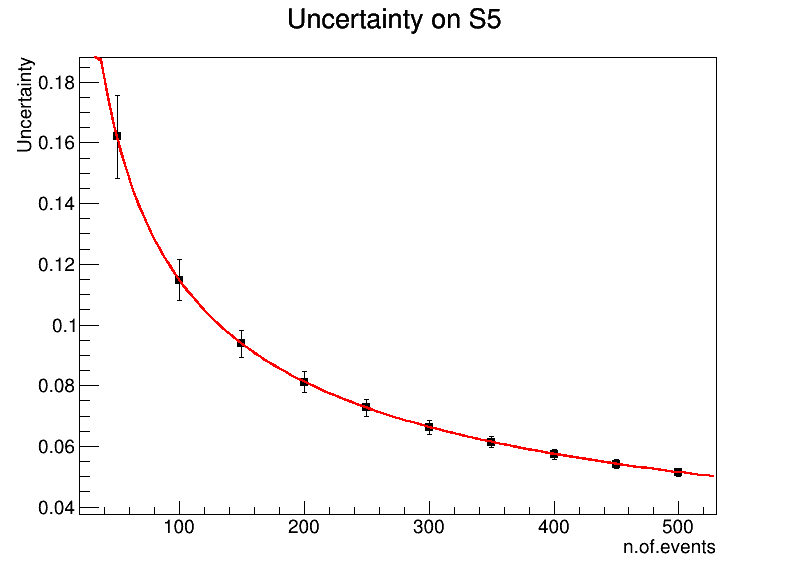
\includegraphics[width=0.8\textwidth]{figs/Q2_5_6_S5.png}
               % \caption{Uncertainty on $S_5$}
                 \end{subfigure}
        \begin{subfigure}[b]{0.45\textwidth}
                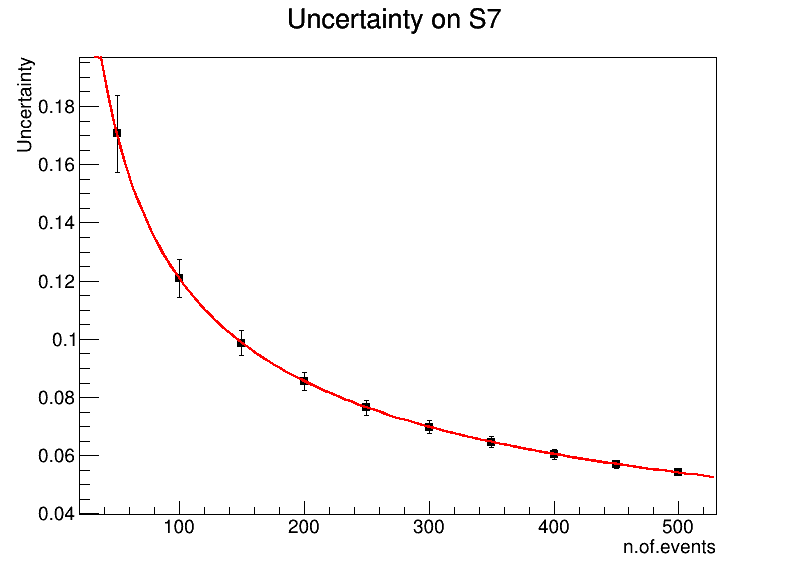
\includegraphics[width=0.8\textwidth]{figs/Q2_5_6_S7.png}
              %\caption{Uncertainty on $S_7$}
                 \end{subfigure}
       \caption{Uncertainty on PDF parameters as a function of number of events. Red curve represents a fit to $f(x)=\dfrac{\alpha}{\sqrt{x}}$ function.}
        \label{errors}
\end{figure}\\
The errors as a function of number of signal events are given in~\ref{errors}. As can be see errors follow strictly the $\sqrt{n}$ law. We performed also the fit to the same toys. For low number of events we observed significant biases. For the high number of signal events we observed  errors coming from fit to be $5-15\%$ smaller then  the ones obtained by method of moments. 


\bibliography{references}

\end{document}
